%=====================================
%    この tex ファイルは『ふきよせ』
%    の記事作成テンプレートです. 
%=====================================

% -----------------------
% preamble
% -----------------------
% ここから本文 (\begin{document}) までの
% ソースコードに変更を加えた場合は
% 編集者まで連絡してください. 
% Don't change preamble code yourself. 
% If you add something
% (usepackage, newtheorem, newcommand, renewcommand),
% please tell it 
% to the editor of institutional paper of RUMS.

% ------------------------
% documentclass
% ------------------------
\documentclass[11pt, a4paper, dvipdfmx]{jsarticle}

% ------------------------
% usepackage
% ------------------------
\usepackage{algorithm}
\usepackage{algorithmic}
\usepackage{amscd}
\usepackage{amsfonts}
\usepackage{amsmath}
\usepackage[psamsfonts]{amssymb}
\usepackage{amsthm}
\usepackage{ascmac}
\usepackage{color}
\usepackage{enumerate}
\usepackage{fancybox}
\usepackage[stable]{footmisc}
\usepackage[dvips]{graphicx}
\usepackage{listings}
\usepackage{mathrsfs}
\usepackage{mathtools}
\usepackage{otf}
%\usepackage{physics}
\usepackage{pifont}
\usepackage{proof}
\usepackage{subfigure}
\usepackage{thmbox}
\usepackage{tikz}
\usepackage{verbatim}
\usepackage[all]{xy}

\usetikzlibrary{cd}



% ================================
% パッケージを追加する場合のスペース 

%=================================


% --------------------------
% theoremstyle
% --------------------------
\theoremstyle{definition}

% --------------------------
% newtheoem
% --------------------------

% 日本語で定理, 命題, 証明などを番号付きで用いるためのコマンドです. 
% If you want to use theorem environment in Japanece, 
% you can use these code. 
% Attention!
% All theorem enivironment numbers depend on 
% only section numbers.
\theoremstyle{definition}
%
%%%%%%%%%%%%%%%%%%%%%%%%%%%%%%%%%%%%%%
%ここにないパッケージを入れる人は,必ずここに記載すること.
%
%%%%%%%%%%%%%%%%%%%%%%%%%%%%%%%%%%%%%%
%ここからはコード表です.
%
\newtheorem{Axiom}{公理}[section]
\newtheorem{Definition}{定義}[section]
\newtheorem{Theorem}{定理}[section]
\newtheorem{Proposition}[Theorem]{命題}
\newtheorem{Lemma}[Theorem]{補題}
\newtheorem{Corollary}[Theorem]{系}
\newtheorem{Example}{例}[section]
\newtheorem{Claim}{主張}[section]
\newtheorem{Property}{性質}[section]
\newtheorem{Attention}{注意}[section]
\newtheorem{Question}{問}[section]
\newtheorem{Problem}{問題}[section]
\newtheorem{Consideration}{考察}[section]
\newtheorem{Alert}{警告}[section]
%%%%%%%%%%%%%%%%%%%%%%%%%%%%%%%%%%%%%%
%
%定義や定理等に番号をつけたくない場合(例えば定理1.1等)は以下のコードを使ってください.
%但し,例えば\Axiom*{}としてしまうと番号が付いてしまうので,必ず \begin{Axiom*} \end{Axiom*}の形で使ってください.

%
%%%%%%%%%%%%%%%%%%%%%%%%%%%%%%%%%%%%%%
%英語で定義や定理を書きたい場合こっちのコードを使うこと.
\newtheorem{Axiom+}{Axiom}[section]
\newtheorem[S]{Defi}[Axiom+]{Definition}
\newtheorem[S]{Thm}[Axiom+]{Theorem}
\newtheorem[S]{Prop}[Axiom+]{Proposition}
\newtheorem[S]{Lem}[Axiom+]{Lemma}
\newtheorem[S]{Ex}[Axiom+]{Example}
\newtheorem[S]{Cor}[Axiom+]{Corollary}
\newtheorem[S]{Prf}[Axiom+]{Proof}
\newtheorem[S]{Rem}[Axiom+]{Remark}
\newtheorem{Claim+}{Claim}
\newtheorem{Property+}{Property}
\newtheorem{Attention+}{Attention}
\newtheorem{Question+}{Question}
\newtheorem{Problem+}{Problem}
\newtheorem{Consideration+}{Consideration}
\newtheorem{Alert+}{Alert}
%
%
% ----------------------------
% commmand
% ----------------------------
% 執筆に便利なコマンド集です. 
% コマンドを追加する場合は下のスペースへ. 

% 集合の記号 (黒板文字)
\newcommand{\NN}{\mathbb{N}}
\newcommand{\ZZ}{\mathbb{Z}}
\newcommand{\QQ}{\mathbb{Q}}
\newcommand{\RR}{\mathbb{R}}
\newcommand{\CC}{\mathbb{C}}
\newcommand{\PP}{\mathbb{P}}
\newcommand{\KK}{\mathbb{K}}


% 集合の記号 (太文字)
\newcommand{\nn}{\mathbf{N}}
\newcommand{\zz}{\mathbf{Z}}
\newcommand{\qq}{\mathbf{Q}}
\newcommand{\rr}{\mathbf{R}}
\newcommand{\cc}{\mathbf{C}}
\newcommand{\pp}{\mathbf{P}}
\newcommand{\kk}{\mathbf{K}}

% 特殊な写像の記号
\newcommand{\ev}{\mathop{\mathrm{ev}}\nolimits} % 値写像
\newcommand{\pr}{\mathop{\mathrm{pr}}\nolimits} % 射影

% スクリプト体にするコマンド
%   例えば {\mcal C} のように用いる
\newcommand{\mcal}{\mathcal}

% 花文字にするコマンド 
%   例えば {\h C} のように用いる
\newcommand{\h}{\mathscr}

% ヒルベルト空間などの記号
\newcommand{\F}{\mcal{F}}
\newcommand{\X}{\mcal{X}}
\newcommand{\Y}{\mcal{Y}}
\newcommand{\Hil}{\mcal{H}}
\newcommand{\RKHS}{\Hil_{k}}
\newcommand{\Loss}{\mcal{L}_{D}}
\newcommand{\MLsp}{(\X, \Y, D, \Hil, \Loss)}

% 偏微分作用素の記号
\newcommand{\p}{\partial}

% 角カッコの記号 (内積は下にマクロがあります)
\newcommand{\lan}{\langle}
\newcommand{\ran}{\rangle}



% 圏の記号など
\newcommand{\Set}{{\bf Set}}
\newcommand{\Vect}{{\bf Vect}}
\newcommand{\FDVect}{{\bf FDVect}}
\newcommand{\Ring}{{\bf Ring}}
\newcommand{\Ab}{{\bf Ab}}
\newcommand{\Mod}{\mathop{\mathrm{Mod}}\nolimits}
\newcommand{\CGA}{{\bf CGA}}
\newcommand{\GVect}{{\bf GVect}}
\newcommand{\Lie}{{\bf Lie}}
\newcommand{\dLie}{{\bf Liec}}



% 射の集合など
\newcommand{\Map}{\mathop{\mathrm{Map}}\nolimits}
\newcommand{\Hom}{\mathop{\mathrm{Hom}}\nolimits}
\newcommand{\End}{\mathop{\mathrm{End}}\nolimits}
\newcommand{\Aut}{\mathop{\mathrm{Aut}}\nolimits}
\newcommand{\Mor}{\mathop{\mathrm{Mor}}\nolimits}

% その他便利なコマンド
\newcommand{\dip}{\displaystyle} % 本文中で数式モード
\newcommand{\e}{\varepsilon} % イプシロン
\newcommand{\dl}{\delta} % デルタ
\newcommand{\pphi}{\varphi} % ファイ
\newcommand{\ti}{\tilde} % チルダ
\newcommand{\pal}{\parallel} % 平行
\newcommand{\op}{{\rm op}} % 双対を取る記号
\newcommand{\lcm}{\mathop{\mathrm{lcm}}\nolimits} % 最小公倍数の記号
\newcommand{\Probsp}{(\Omega, \F, \mathbb{P})} 
\newcommand{\argmax}{\mathop{\rm arg~max}\limits}
\newcommand{\argmin}{\mathop{\rm arg~min}\limits}





% ================================
% コマンドを追加する場合のスペース 

% =================================





% ---------------------------
% new definition macro
% ---------------------------
% 便利なマクロ集です

% 内積のマクロ
%   例えば \inner<\pphi | \psi> のように用いる
\def\inner<#1>{\langle #1 \rangle}

% ================================
% マクロを追加する場合のスペース 

%=================================





% ----------------------------
% documenet 
% ----------------------------
% 以下, 本文の執筆スペースです. 
% Your main code must be written between 
% begin document and end document.
% ---------------------------

\title{Generative Adversarial Networks and their theoretical Analysis}
\author{理工学部 数理科学科 小泉 孝弥}
\date{}
\begin{document}
\maketitle


%===============================================
\section{Introduction}
皆さんは, GANというものを知っているだろうか. GANとは敵対的生成ネットワーク(Generative Adversarial Networks)のこと
であり, 2014年に登場した人工知能の技術である. 「敵対的」という単語がついている通り, 2つの
ニューラルネットワークという関数を競わせることで, 学習させていく手法である. なお, 前提知識
は数学科学部3回生程度の知識である. 
\section{Fundermetal concepts of Machine Learning}
この節では機械学習の数学的な定式化を行う. $d$, $m$を自然数とする.
\begin{Defi}[仮説空間, 仮説]
    $\X\subset\RR^d$から$\Y\subset\RR^m$へのなんらかの条件を満たす写像の集まりのことを仮説空間
    といい$\Hil$と表記する. すなわち,
    \begin{align*}
        \Hil = \{f:\X\to\Y\mid f\text{ が満たす条件}\}
    \end{align*}
    である. (条件の具体例は後に述べる). 仮設空間$\Hil$の元のことを仮説(またはモデル)と呼ぶ.
    また, この時の$\X$を入力空間, $\Y$を出力空間と呼ぶ. 
\end{Defi}
\begin{Defi}[データ]
    $(\Omega, \mathcal{F}, \mathbb{P})$を確率空間, $\rho$を$\X\times\Y$上の確率分布とする.
    $\{(X_n, Y_n)\}_{n = 1}^{N}$を$\rho$に従う独立な確率変数列とした時, $\{(X_n, Y_n)\}_{n = 1}^{N}$の観測値$\{(X_n(\omega), Y_n(\omega))\}_{n = 1}^{N}$
    のことを教師ありデータと呼び, $\{(x_n, y_n)\}_{n = 1}^{N}$と表記する. 同様に, $\rho$を$\X$上の確率分布とし,
    $\{X_n\}_{n = 1}^{N}$を$\rho$に従う独立な確率変数列とした時, $\{X_n\}_{n = 1}^{N}$の観測値$\{X_n(\omega)\}_{n = 1}^{N}$
    のことを教師なしデータと呼び$\{x_n\}_{n = 1}^{N}$と表記する. また, 両者をまとめてデータと呼び$D$で表す.
\end{Defi}
\begin{Defi}[汎化誤差, 損失関数]
    $\Hil$を仮説空間, $(\Omega, \mathcal{F}, \mathbb{P})$を確率空間, $\rho$をデータの確率分布とする.
    この時, 汎化誤差$\ell:\Hil\to\RR$を, 
    \begin{equation*}
        l(f_{w}) = \mathbb{E}_{(X, Y)\sim\rho}[\ell(f_{w}(X), Y)]
    \end{equation*}
    と定義する. ここで, $\ell:\Y\times\Y\to\RR$は損失関数と呼ばれる凸関数である. 
\end{Defi}
\begin{Ex}[損失関数]
    ここで, よく使われる損失関数の例をいくつか述べておく. 
    \begin{enumerate}
        \item 2乗損失関数 $\ell(y_1, y_2) = (y_1 - y_2)^2$
        \item 交差エントロピー誤差 $\ell(y_1, y_2) = -y_2\log y_1$
    \end{enumerate}
\end{Ex}
汎化誤差が最小となるような$f\in\Hil$を求めることが機械学習の目標である. しかし, 一般にデータの分布は未知であるため
この式を解くことができない. そこで、損失関数というものを定義し, それを最適化することを考える.
\begin{Defi}[経験損失関数]
    $\Hil$を仮説空間とする. $\Hil$から$\RR$への写像$\Loss:\Hil\to\RR$を経験損失関数(Loss function)と呼ぶ.
\end{Defi}
\begin{Defi}[機械学習空間(ML空間)]
    $D$をデータ, $\Hil$を仮説空間, $\Loss$を経験損失関数とする. 
    この時5つ組$\MLsp$を機械学習空間(Machine Learning space)あるいは, ML空間という.
\end{Defi}
\begin{Defi}[学習, 最適仮説]
    $\Hil$を仮設空間, $\Loss:\Hil\to\RR$を経験損失関数とする. 経験損失関数が最大または, 最小となるような
    $f^*\in\Hil$を求めること\footnote{機械学習においては厳密に損失関数が最大・最小となる関数が得られるとは限らないが, そのような関数を求めることも学習の定義に含めるものとする. }を学習といい, $f^*\in\Hil$を最適仮説と呼ぶ.
\end{Defi}
\begin{Defi}[機械学習]
    機械学習空間$\MLsp$上での学習を機械学習という. 特に, $D$が教師ありデータの時, 教師あり機械学習と呼び, 
    教師なしデータの時, 教師なし機械学習と呼ぶ.
\end{Defi}
\begin{Rem}[訓練データとテストデータ]
    機械学習を行う際は, データ$D$を全て使って学習させるのではなく, 
    データを訓練データ$D_{\text{Train}}$とテストデータ$D_{\text{Test}}$に分ける. 
    訓練データはモデルの学習に用いて, テストデータはモデルの精度の確認のために用いる. 
\end{Rem}
\section{Some Examples}
前節では, 機械学習の抽象的な枠組みを紹介したが, この説では機械学習空間の具体例を述べる.
$D = \{(x_i, y_i)\}_{i = 1}^{N}\subset\X\times\Y$を教師ありデータとする.

\subsection{単回帰分析・重回帰分析}
最初に機械学習の最も基本的なモデルである重回帰分析を紹介する. 
\begin{Ex}[重回帰分析]
    機械学習空間$\MLsp$を以下のように定義する.\\
    $\X = \RR^d(N\geq d)$, $\Y = \RR$, 
    \begin{align*}
        \Hil &= \{f:\X\to\Y\mid f(x) = W^{\top}x + b, W\in\RR^{d}, b\in\RR\},\\
        \Loss(f) &= \sum_{i = 1}^{N}|f(x_i) - y_i|^2.
    \end{align*}
    この機械学習空間$\MLsp$上で
    \begin{align*}
        \argmin_{f\in\Hil}\Loss(f)
    \end{align*}
    を求める問題を重回帰分析という. $X\in\RR^{N\times(d + 1)}$を
    \begin{align*}
        X = \begin{pmatrix}
            1 & x_{11} & x_{12} & \cdots & x_{1d}\\
            1 & x_{21} & x_{22} & \cdots & x_{2d}\\
            \vdots & \vdots & \vdots & \ddots & \vdots\\
            1 & x_{N1} & x_{N2} & \cdots & x_{Nd}
        \end{pmatrix}
    \end{align*}
    と定義し, $\mathbf{y} = (y_{1}, y_{2}, \cdots, y_{N})^{\top}\in\RR^{N}$とする. この時, $\mathbf{rank}(X) = d + 1$ならば, 
    最適仮説$f^*\in\Hil$は$[b~W] = (X^\top X)^{-1}X^\top\mathbf{y}$とすれば
    \begin{align*}
        f^{*}(x) = [b~W]^{\top}x
    \end{align*}
    である. なお, $d = 1$の時, 重回帰分析を単回帰分析という.
\end{Ex}
\subsection{線形回帰}
前小節で定義した重回帰分析は線形的なデータにしか適応できなかった. それを
基底関数と呼ばれる関数列を定義する事で, 非線形データにも対応することができる.
\begin{Defi}[基底関数]
    $\X$を入力空間とし, 任意に$d\in\NN$をとる. $\X$上の連続関数列$\{\phi_{n}\}_{n = 1}^{d}\subset C(\X, \X)$
    が一次独立であるとき, $\Phi = (\phi_1, \phi_2, \cdots, \phi_d)^{\top}:\X\to\X^{d}$を基底関数(basis function)と呼ぶ.
\end{Defi}
\begin{Ex}[多項式回帰]
    機械学習空間$\MLsp$を以下のように定義する.\\
    $\X = \RR, \Y = \RR$, 
    \begin{align*}
        \Hil &= \{f:\X\to\Y\mid f(x) = W^{\top}\Phi(x), W\in\RR^{d + 1}\},\\
        \Loss(f) &= \sum_{i = 1}^{N}|f(x_i) - y_i|^2.
    \end{align*}
    ここで, $\phi_{n}(x) = x^{n}$, $n\in\{0, 1, \cdots, d\}$とする.\\
    この機械学習空間$\MLsp$上で
    \begin{align*}
        \argmin_{f\in\Hil}\Loss(f)
    \end{align*}
    を求める問題を多項式回帰という. $X = [\Phi(x_1), \Phi(x_{2}), \cdots, \Phi(x_N)]^{T}\in\RR^{N\times d}$とし, 
    $\mathbf{y} = (y_{1}, y_{2}, \cdots, y_{N})^{T}\in\RR^{N}$とする. この時, 最適仮説$f^{*}$は
    重回帰分析と同様に$W = (X^\top X)^{-1}X^\top\mathbf{y}$とすれば
    \begin{align*}
        f^{*}(x) = W^{\top}x
    \end{align*}
    である. 
\end{Ex}
\begin{Rem}[ハイパーパラメータと学習パラメータ]
    多項式回帰の多項式の次数$d\in\NN$や基底関数$\{\phi_{n}\}_{n = 1}^{d}$のように
    コンピュータに学習させるのではなく, 機械学習モデルの設計者が設定するパラメータのことを
    ハイパーパラメータと呼ぶ. 一方, $W\in\RR^{d + 1}$のように, データからコンピュータが自動で学習
    するパラメータのことを学習パラメータと呼び, $\Theta$と表す.
\end{Rem}
\subsection{過学習と正則化}
前節の多項式回帰で学習を行うと以下のグラフのように, 訓練データに過剰適合してしまい, 未知のデータに関しての汎化性能
が小さくなってしまうことを過学習(overfitting)という. 
\begin{figure}[H]
    \centering
    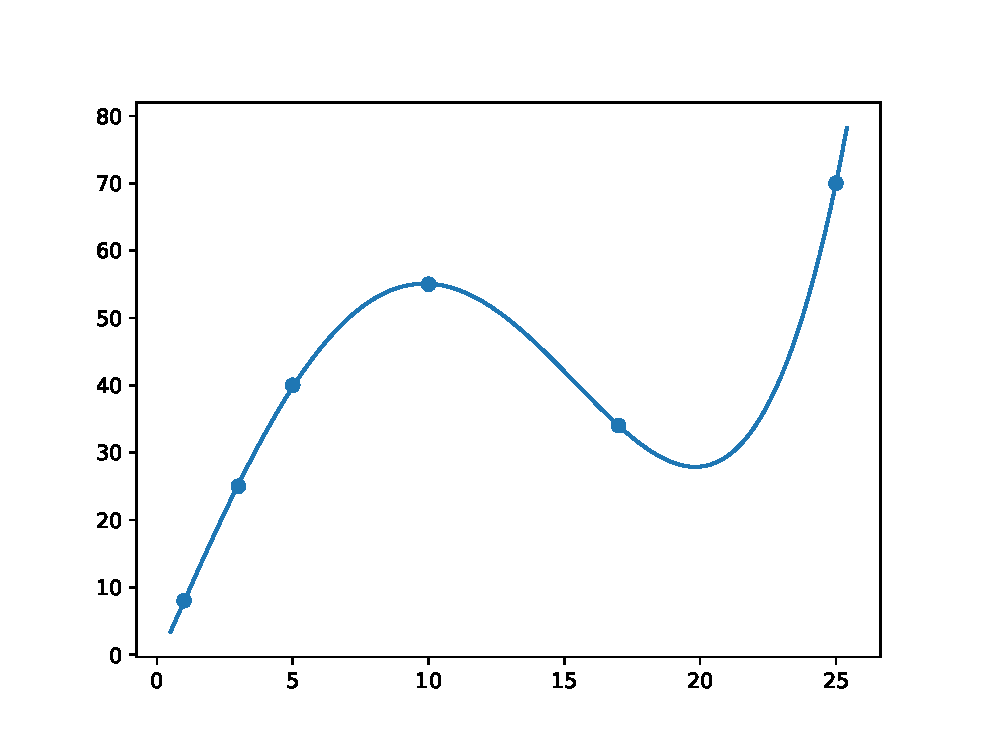
\includegraphics[width = 9.0cm]{Images/overfitting_PR.eps}
    \caption{$d = 4$の時の多項式回帰の過学習}
\end{figure}
過学習を防ぐための手法が正則化である.
\begin{Defi}[正則化]
    $\Loss:\Hil\to\RR$を損失関数とする. $\Loss^{R} := \Loss + L^{R}$とする.
    この時, $\Loss^{R}$を$\Loss$の正則化と呼び, $L^R:\Theta\to\RR$を正則化項と呼ぶ.
\end{Defi}
\begin{Ex}[Ridge正則化多項式回帰]
    $\lambda\in\RR^{+}\coloneqq\{x\in\RR\mid x\geq0\}$, $d\in\NN$を任意にとる.機械学習空間$\MLsp$を以下のように定義する.\\
    $\X = \RR, \Y = \RR$, 
    \begin{align*}
        \Hil &= \{f:\X\to\Y\mid f(x) = W^{\top}\Phi(x), W\in\RR^{d + 1}\},\\
        \Loss(f) &= \sum_{i = 1}^{N}|f(x_i) - y_i|^2+\lambda W^\top W.\hspace{10pt} (W\text{は$f$のパラメータ})
    \end{align*}
    ここで, $\phi_{n}(x) = x^{n}$, $n\in\{0, 1, \cdots, d\}$とする($\lambda W^{\top}W$が正則化項である).\\
    この機械学習空間$\MLsp$上で
    \begin{align*}
        \argmin_{f\in\Hil}\Loss(f)
    \end{align*}
    を求める問題をRidge正則化多項式回帰という. 通常の多項式回帰の時と同様に, $X = [\phi_{1}(x_1), \phi_{2}(x_{2}), \cdots, \phi_{N}(x_N)]^{\top}\in\RR^{N\times d}$とし, 
    $\mathbf{y} = (y_{1}, y_{2}, \cdots, y_{N})^{\top}\in\RR^{N}$とする. この時, 最適仮説$f^{*}$は
    $W = (X^\top X + \lambda I)^{-1}X^\top\mathbf{y}$とすれば
    \begin{align*}
        f^{*}(x) = W^{\top}x
    \end{align*}
    である. 
\end{Ex}
正則化の結果が以下のグラフである.
\begin{figure}[H]
    \centering
    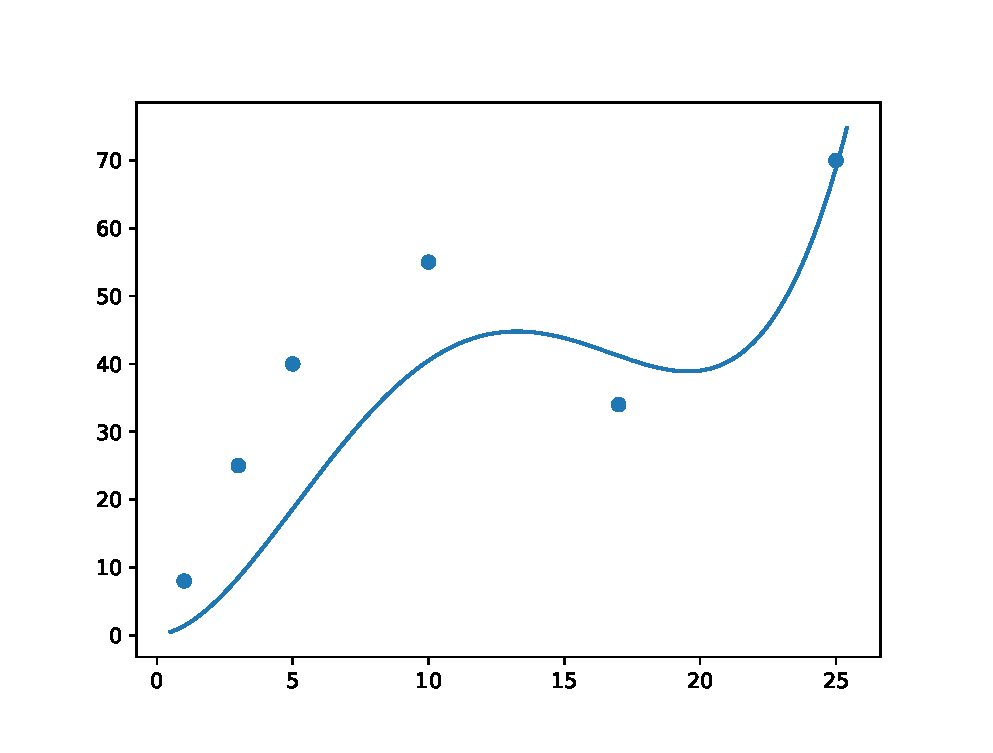
\includegraphics[width = 7.5cm]{Images/regulared_PR.eps}
    \caption{$\lambda = 700$, $d = 4$の時のRidge正則化多項式回帰}
\end{figure}
このように正則化をすることで, パラメータが大きくなりすぎることを防ぐことで過学習を防ぐことができる.
\begin{Rem}[未学習について]
    正則化を行う際にパラメータ\footnote{正則化パラメータという.}$\lambda\in\RR^+$は自分で
    決める必要がある. その際に$\lambda$の値を大きくしすぎると未学習(underfitting)という問題が発生する.
    未学習とは訓練データに対してモデルが十分に適合できていないことをいう.
    \begin{figure}[H]
        \centering
        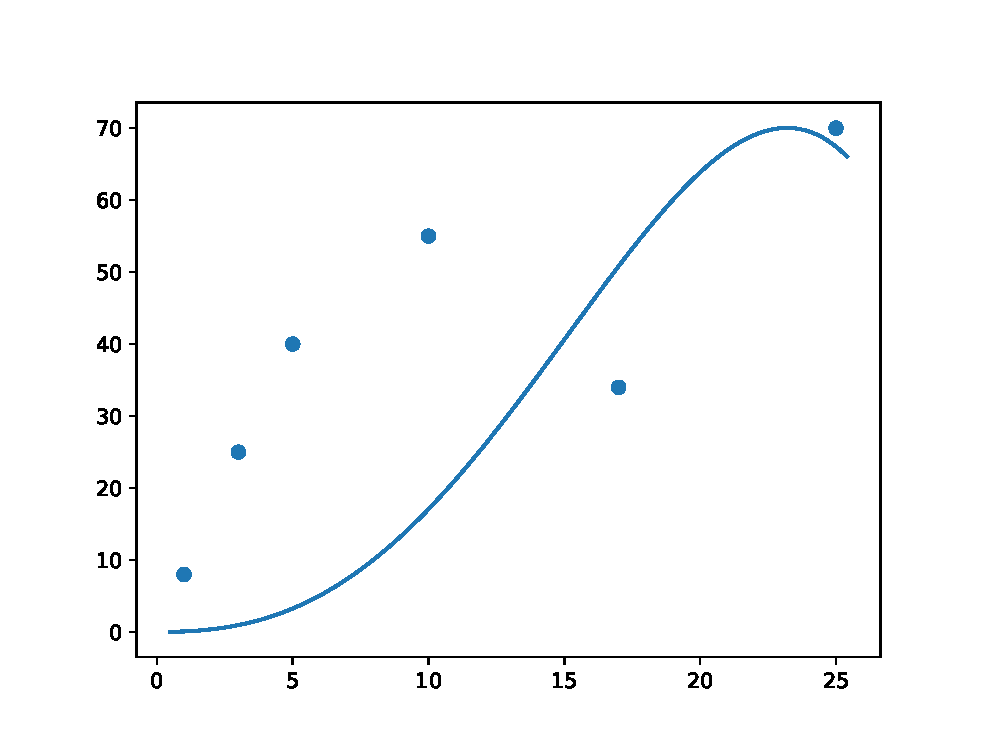
\includegraphics[width=7.5cm]{Images/underfitting_PR.eps}
        \caption{$\lambda = 30000$, $d = 4$の時のRidge正則化多項式回帰の未学習}
    \end{figure}
    このように, 正則化パラメータは適切に選ぶことが大切である. 
\end{Rem}
\subsection{ロジスティック回帰と勾配降下法}
最後の具体例として, ロジスティック回帰を紹介する. 
ロジスティック回帰は分類問題を解くための手法の1つである.
まず, 実数値ベクトルを確率に変換するソフトマックス関数および, one-hotベクトルというものを
導入する. 
\begin{Defi}[ソフトマックス関数]
    $\psi:\RR^d\to\RR^d$を以下で定義する.
    \begin{align*}
        \psi(x)_{i} = \frac{\exp(x_i)}{\sum_{k = 1}^d\exp(x_k)}
    \end{align*}
    この時, $\psi$をソフトマックス関数と呼ぶ.
\end{Defi}
\begin{Defi}[one-hotベクトル]
    $y\in\RR^m$が第$c\in\{1, 2, \cdots, m\}$成分が1であり, 残りの成分が0である時, 
    $y$をone-hotベクトルという.
\end{Defi}
\begin{Ex}[$m$値分類ロジスティック回帰]
    機械学習空間$\MLsp$を以下のように定義する.\\
    $\X=\RR^d$, $\Y = \RR^m$, 
    \begin{align*}
        \Hil &= \{f:\X\to\Y\mid f(x) = \psi(Wx + b), W\in\RR^{m\times d}, b\in\RR^m\},\\
        \Loss(f) &= -\sum_{n = 1}^{N}\sum_{k = 1}^{m}y_{nk}\log f(x_n)_{k},
    \end{align*}
    ここで$\psi:\RR^m\to\RR^m$はソフトマックス関数であり, $y_{n}$はone-hotベクトルである.\\
    この機械学習空間$\MLsp$上で
    \begin{align*}
        \argmin_{f\in\Hil}\Loss(f)
    \end{align*}
    を求める問題を$m$値分類ロジスティック回帰という.
\end{Ex}
先ほどまでは, 損失関数の最小値を解析的に求めていたが, 今回の損失関数の最小値を解析的に求めることはせず,
勾配降下法という連続最適化アルゴリズムを用いて求めることにする. 勾配降下法とは$C^{1}$関数$F$の
最小値を求めるためのアルゴリズムである.
\begin{algorithm}[H]
    \caption{Gradient Decent}
    \begin{algorithmic}
        \REQUIRE F: $C^1$ function on $\RR^{d}$
        \REQUIRE $0<\alpha<1$ : learning rate 
        \REQUIRE $\theta$: Initial parameter vector
        \STATE $\theta\leftarrow\theta_{0}$
        \WHILE{$\theta$ not converged} 
        \STATE $\theta\leftarrow\theta - \alpha\nabla F(\theta)$ 
        \ENDWHILE
        \RETURN $\theta$
    \end{algorithmic}
\end{algorithm}
\begin{Ex}[2次関数における勾配降下法]
    $y = x^2$において勾配降下法を適応した結果を以下の図と表に示す.
    本来の最適値である$x = 0$に近づいているのが分かる.
    \begin{figure}[H]
        \centering
        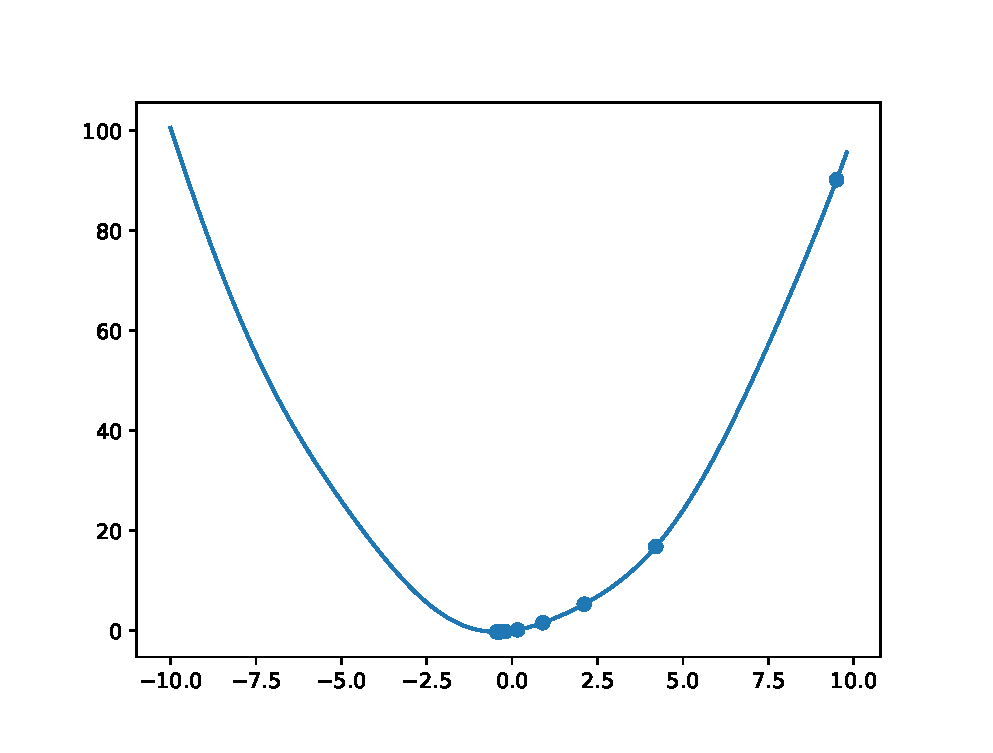
\includegraphics[width = 8.5cm]{Images/Gradient_Decent.eps}
        \caption{$\alpha = 0.001$とした時の勾配降下法の結果.}
    \end{figure}
    \begin{table}[H]
        \centering
        \begin{tabular}{|c|c|c|c|c|c|c|c|c|c|c|}\hline
            イテレーション数 & 0 & 400 & 800 & 1200 & 1600 & 2000 & 2400 & 2800 & 3200 & 3600\\\hline
            $\theta$の値 & 9.50 & 4.27 & 1.91 & 0.86 & 0.39 & 0.17 & 0.08 & 0.03 & 0.02 & 0.01\\\hline
        \end{tabular}
        \caption{値の詳細}
    \end{table}
\end{Ex}
\subsection{MNISTでの実験}
MNISTとは下記のような0から9までの自然数が書かれた$28\times28$ピクセル画像のデータセットの名前である. 
今回は, $m$値分類のロジスティック回帰を用いて、画像に書かれている文字を予測する問題を
考える. ロジスティック回帰の損失関数$\Loss$を勾配降下法を用いて最小化するため, まずは損失関数の勾配を計算する.
ここで, $\Hil\simeq\RR^{m\times d + 1}$だから, $\Loss$を$\RR^{m\times d + 1}$上の関数と考える.\
\begin{figure}[htbp]
    \begin{minipage}{0.32\hsize}
        \centering
        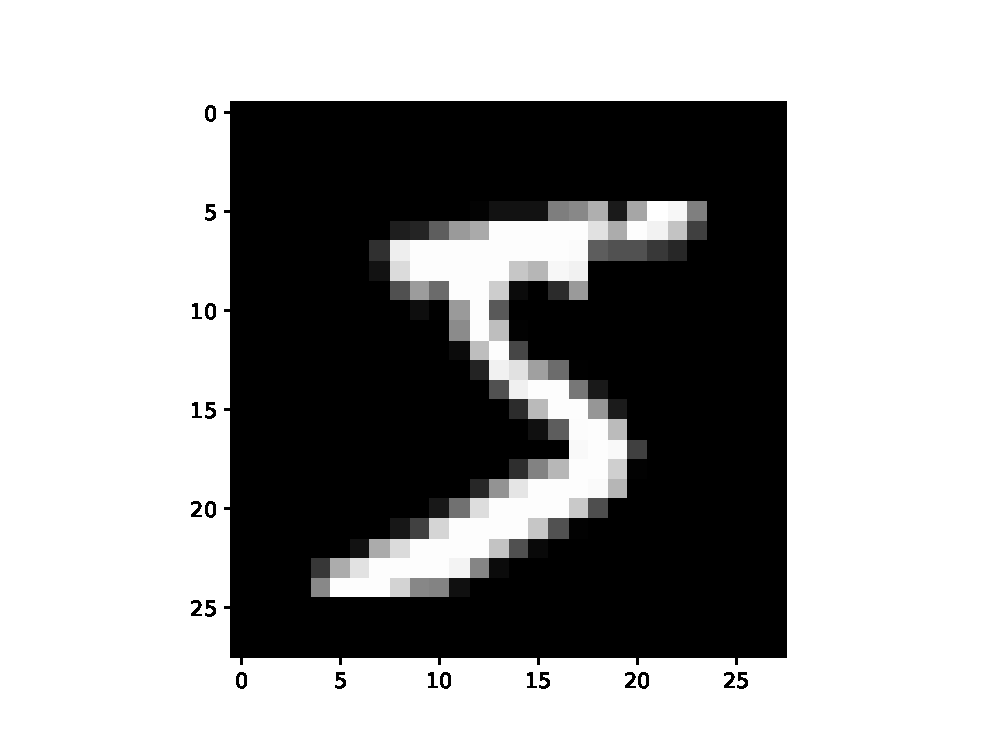
\includegraphics[width = 5.3cm]{Images/MNIST_sample1.eps}
        \caption{数字の5}
    \end{minipage}
    \begin{minipage}{0.32\hsize}
        \centering
        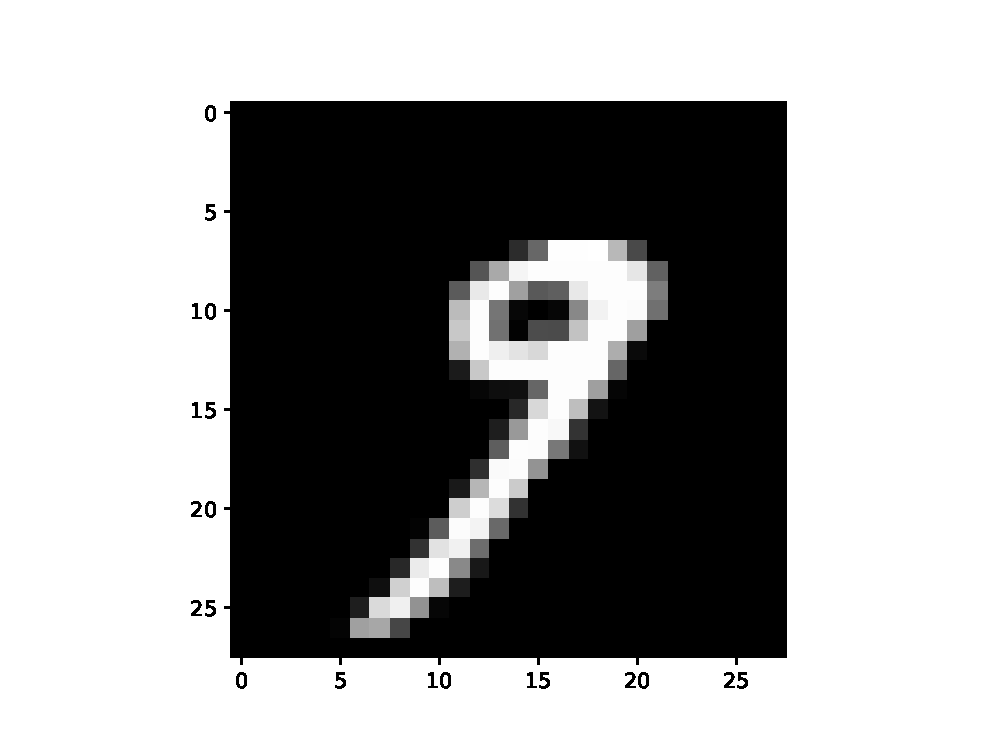
\includegraphics[width = 5.3cm]{Images/MNIST_sample2.eps}
        \caption{数字の9}
    \end{minipage}
    \begin{minipage}{0.32\hsize}
        \centering
        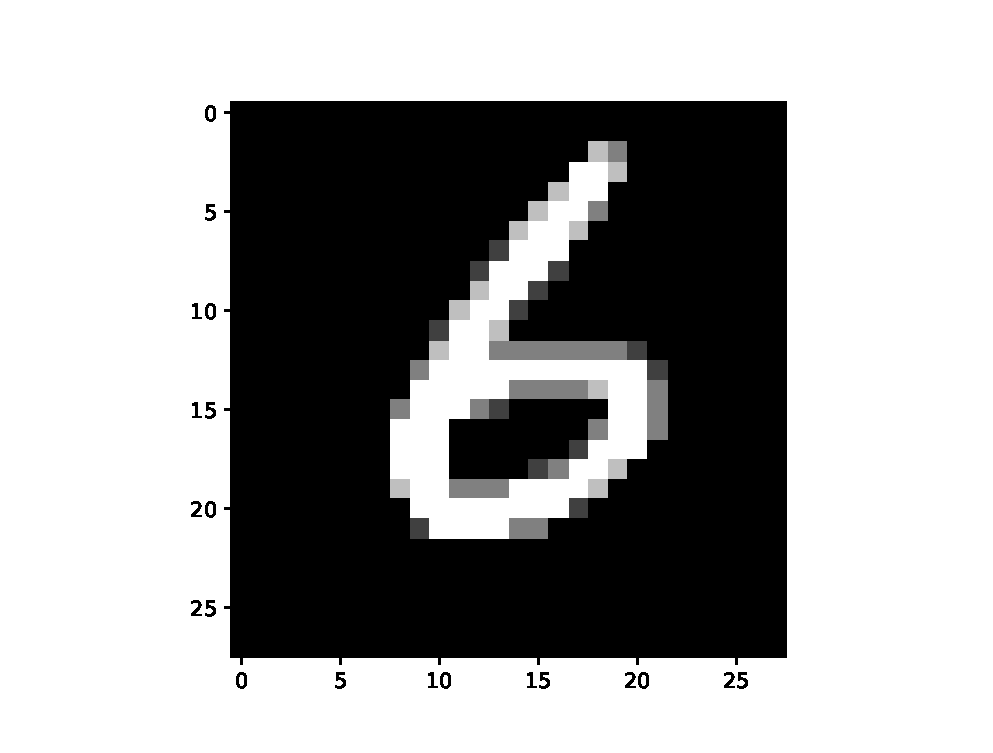
\includegraphics[width = 5.3cm]{Images/MNIST_sample3.eps}
        \caption{数字の6}
    \end{minipage}
\end{figure}
\begin{Lem}[$\cite{MLR}$]\label{test}
    任意の$i\in\{1, 2, \cdots, m\}, j\in\{1, 2, \cdots, d\}$に対して以下が成立する.
    \begin{align*}
        \frac{\partial\Loss}{\partial w_{ij}} &= -\sum_{n = 1}^{N}\left(y_{ni} - f(x_{n})_{i}\right)x_{nj}\\
        \frac{\partial\Loss}{\partial b_{i}} &= -\sum_{n = 1}^{N}(y_{ni} - f(x_{n})_{i})
    \end{align*}
\end{Lem}
この補題$\Ref{test}$より, 
\begin{align*}
    \frac{\partial\Loss}{\partial W} &= - 
    \begin{pmatrix}
        \sum_{n = 1}^{N}\left(y_{n1} - f(x_{n})_{1}\right)x_{n1} & \cdots & \sum_{n = 1}^{N}\left(y_{n1} - f(x_{n})_{1}\right)x_{nd}\\
        \vdots & \ddots & \vdots\\
        \sum_{n = 1}^{N}\left(y_{nm} - f(x_{n})_{m}\right)x_{n1} & \cdots & \sum_{n = 1}^{N}\left(y_{nm} - f(x_{n})_{m}\right)x_{nd}
    \end{pmatrix}\\ 
    & = - 
    \begin{pmatrix}
        y_{11} - f(x_1)_1 & \cdots & y_{N1} - f(x_N)_m\\
        \vdots & \ddots & \vdots\\
        y_{1m} - f(x_1)_m & \cdots & y_{Nm} - f(x_N)_m
    \end{pmatrix}
    \begin{pmatrix}
        x_{11} & \cdots & x_{1d} \\
        \vdots & \ddots & \vdots \\
        x_{N1} & \cdots & x_{Nd}
    \end{pmatrix}\\
    &= -(Y - F)X^{\top},
\end{align*}
ここで, $X = [x_{1}, x_{2}, \cdots, x_{N}]$, $Y = [y_1, y_2, \cdots, y_N]$, $F = [f(x_1), f(x_2), \cdots, f(x_N)]$である. 
また, この計算より$\mathbf{1} = [1, 1, \cdots, 1]^{\top}\in\RR^{N\times 1}$とすれば,
\begin{align*}
    \frac{\partial\Loss}{\partial b} = -(Y - F)\mathbf{1}
\end{align*}
もいえる. これらを用いて学習した結果を以下に示す. また, この例からもわかるように機械学習においてパラメータの次元は
非常に高次元なものとなる. (今回は$10\times784 + 10 = 7850$次元).
\begin{figure}[H]
    \centering
    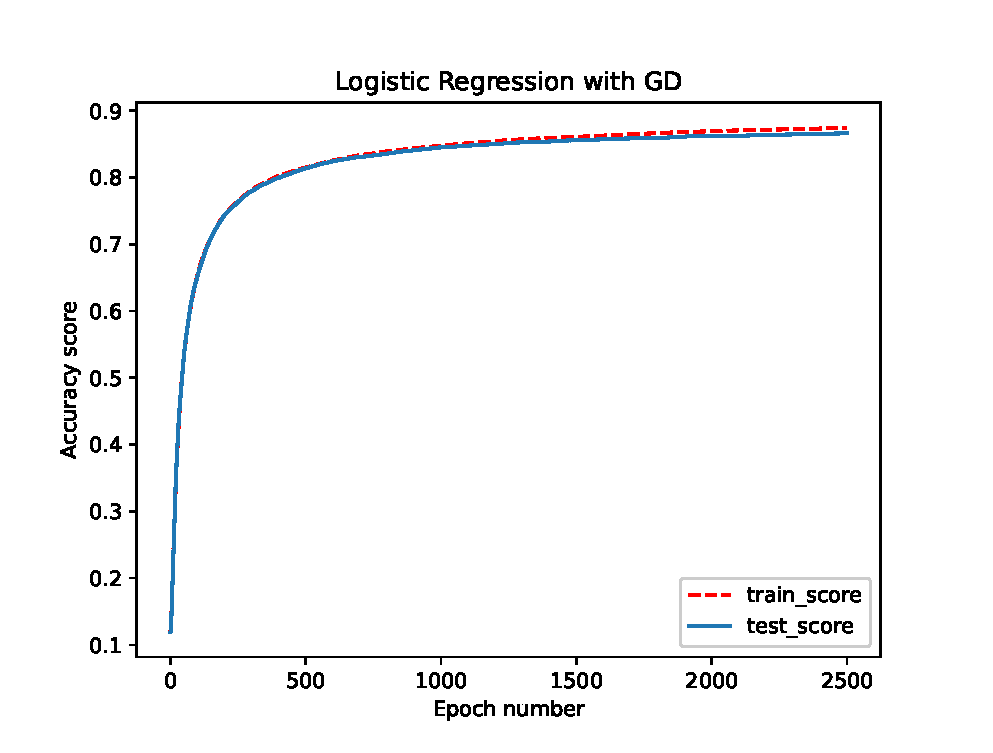
\includegraphics[width = 7.0cm]{Images/MNIST_Experiment.eps}
    \caption{$\alpha = 0.0001$とした時の, MNSIT実験の結果}
\end{figure}
この例からもわかる通り, 機械学習において$\RR^d$上の関数を学習するのではなく
意味のある$\RR^d$の部分集合上の関数(今回なら$[0, 1]^d$)を学習していることがほとんどである.
\section{Deep Learning}
ここから、高い表現能力を持つとされるニューラルネットワークについて説明する. 
ニューラルネットワークとはアフィン変換と活性化関数と呼ばれる関数の合成関数である. 前節と同様に
$D = \{(x_i, y_i)\}_{i = 1}^{N}\subset\X\times\Y$を教師ありデータとする.
\subsection{Neural Network}
\begin{Defi}[活性化関数]
    $\sigma:\RR^{d}\to\RR^{d}$を非線形かつ, Lipschitz連続な関数とする. 
    この時, $\sigma$を活性化関数(activation function)という.
\end{Defi}
\begin{Ex}[活性化関数の具体例]
    活性化関数の具体例をいくつか述べる. 
    \begin{align*}
        \sigma(x)_{i} &= \frac{1}{1 + \exp(-x_{i})},\\
        \text{ReLU}(x)_{i} &= \max(x_{i}, 0).
    \end{align*}
    $\sigma$をシグモイド関数(sigmoid function), $\text{ReLU}$を正規化線形関数(Rectified Linear Unit)
    という.
\end{Ex}
\begin{Defi}[回帰型ニューラルネットワーク]
    機械学習空間$\MLsp$を以下のように定義する. $L = \{L_{1}, L_{2}, \cdots, L_{K}\}$を自然数列とする.
    $\X = \RR^d$, $\Y = \RR$, 
    \begin{align*}
        \Hil &= \left\{f:\X\to\Y~\middle|
        \begin{array}{l}
            f(x) = W^{\top}g_{K}\circ g_{K - 1}\circ\cdots\circ g_{1}(x) + b, g_{i} = \eta(W_{i}x + b_{i})\\
            W_{i}\in\RR^{L_{i}\times L_{i - 1}}, b_{i}\in\RR^{L_{i}}, W\in\RR^{L_{K}}, b\in\RR
        \end{array}
        \right\},\\
        \Loss(f) &= \frac{1}{N}\sum_{i = 1}^{N}|f(x_i) - y_i|^2,
    \end{align*}
    ここで$\eta$は活性化関数である. $f\in\Hil$を回帰型(全結合)ニューラルネットワーク(Full-connected Neural Network for Regression)
    と呼び, 各$g_{i}$を$f$の第$i$層(layer)と呼ぶ.
\end{Defi}
\begin{Defi}[分類型ニューラルネットワーク]
    機械学習空間$\MLsp$を以下のように定義する. $L = \{L_{1}, L_{2}, \cdots, L_{K}\}$を自然数列とする.
    $\X = \RR^d$, $\Y = \RR^{m}$, 
    \begin{align*}
        \Hil &= \left\{f:\X\to\Y~\middle|
        \begin{array}{l}
            f(x) = \psi(W g_{K}\circ g_{K - 1}\circ\cdots\circ g_{1}(x) + b), g_{i} = \eta(W_{i}x + b_{i})\\
            W_{i}\in\RR^{L_{i}\times L_{i - 1}}, b_{i}\in\RR^{L_{i}}, W\in\RR^{m\times L_{K}}, b\in\RR^{m}
        \end{array}
        \right\},\\
        \Loss(f) &= -\sum_{n = 1}^{N}\sum_{k = 1}^{m}y_{nk}\log f(x_n)_{k},
    \end{align*}
    ここで$\eta$は活性化関数, $y_{i}$はone-hotベクトル, $\psi$はソフトマックス関数である. $f\in\Hil$を分類型(全結合)ニューラルネットワーク(Full-connected Neural Network for Classification)
    と呼び, 回帰型の時と同様に各$g_{i}$を$f$の第$i$層と呼ぶ.
\end{Defi}
以下, ニューラルネットと書けば, 分類, 回帰ニューラルネットワークのいずれかを表すものとする. 
\begin{Defi}[深層学習]
    ニューラルネットワークが$K \geq 3$の時に
    \begin{align*}
        \argmin_{f\in\Hil}\Loss(f)
    \end{align*}
    を求める問題を深層学習(Deep Learning)と呼ぶ.
\end{Defi}
\begin{figure}[H]
    \centering
    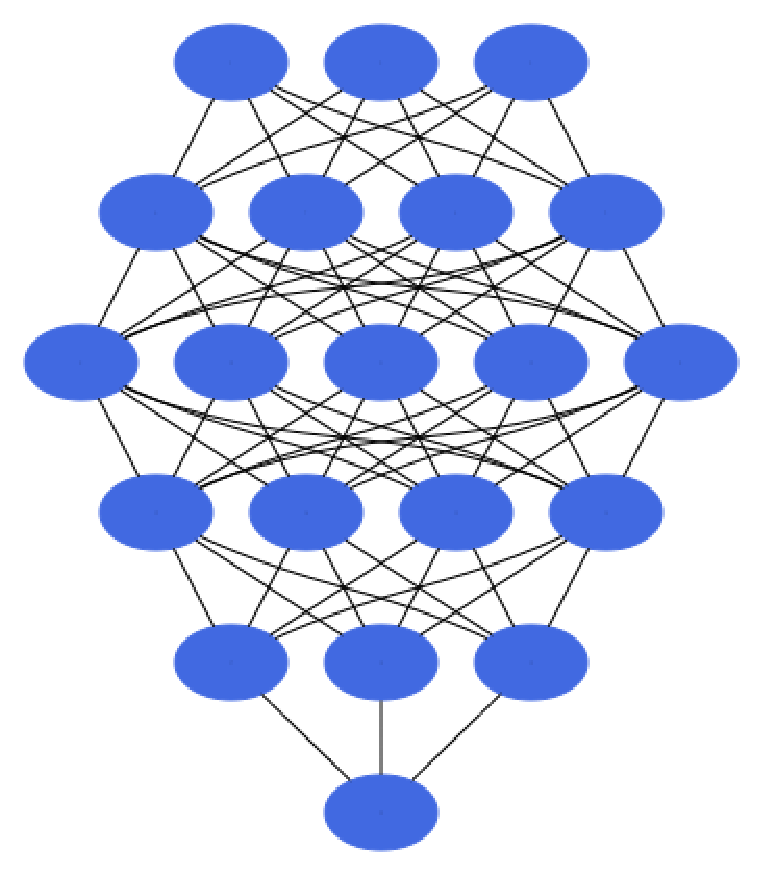
\includegraphics[width = 9.0cm, angle=90]{Images/NN.eps}
    \caption{ニューラルネットワークの図}
\end{figure}
\begin{Rem}[フレームワーク]
    現在はニューラルネットワークを簡単に実装するための深層学習フレームワークという
    ものがいくつか存在する. 代表なものとして, FacebookのPytorchや, GoogleのTensorflowなどがある.
\end{Rem}
\subsection{The Universal Theorem of Neural Network}
冒頭でも述べたが, 深層学習は前説まで紹介してきた機械学習の手法と
比べて, 精度がよくなることが知られている. しかしながら, その数学的な理由については現在も研究途中である. 
一方で, ニューラルネットの表現能力についてはいくつかの成果が出ており, その一つである
普遍性定理を紹介する. 証明については$\cite{UAT}$や$\cite{DUAT}$を見て欲しい.
\begin{Defi}[符号付き測度]
    $(X, \F)$を可測空間とする. $\mu:\F\to\RR$が, 任意の互いに素な$\{A_{n}\}_{n\in\NN}\subset\F$に対して
    \begin{align*}
        \mu\left(\bigcup_{n\in\NN}A_{n}\right) = \sum_{n\in\NN}\mu(A_{n})
    \end{align*}
    を満たすとき, $\mu$を符号付き測度という. 
\end{Defi}
\begin{Defi}[正則Borel測度]
    $(X, \mathcal{O})$を位相空間とする. Borel集合族$\mathcal{B}(X)$上のBorel測度$\mu$が
    \begin{align*}
        \forall A\in\mathcal{B}(X), \mu(A) &= \inf\{\mu(U)\mid U\supset A, U\in\mathcal{O}\} \\
                                           &= \sup\{\mu(K)\mid K\subset A, K\text{ is compact and closed}\}
    \end{align*}
    を満たす時, 正則Borel測度という. 
\end{Defi}
\begin{Defi}[正則符号付きBorel測度]
    $(X, \mathcal{O})$を位相空間とする. $(X, \mathcal{B}(X))$上の符号付き測度$\mu$が
    正則符号付きBorel測度であるとは, 以下で定義される$\mathcal{B}(X)$上の有限測度$\mu^{+}$, $\mu^{-}$が
    共に正則Borel測度になることである.
    \begin{align*}
        \mu^{+}(A) &= \sup\{\mu(B)\mid B\in\mathcal{B}(X), B\subset A\},\\
        \mu^{-}(A) &= -\inf\{\mu(B)\mid B\in\mathcal{B}(X), B\subset A\}.
    \end{align*}
    また, $X$上の正則符号付き測度全体の集合を$M(X)$と表記する.
\end{Defi}
\begin{Defi}[Sigmoidal]
    関数$\sigma:\RR\to\RR$がシグモイド的関数であるとは
    \begin{align*}
        \lim_{t\to+\infty} \sigma(t) = 1\hspace{10pt}\lim_{t\to-\infty} \sigma(t) = 0
    \end{align*}
    を満たすことである.
\end{Defi}
\begin{Thm}[普遍性定理]
    $X\subset\RR^n$をコンパクト連結部分空間とし, $\Hil$を$K = 1$の時の回帰型ニューラルネットの仮説空間とする. 
    この時, 活性化関数$\eta$がシグモイド的関数ならば, 
    \begin{align*}
        \forall f\in C(X), \forall\e> 0, \exists G\in\Hil\text{ s.t. } \sup_{x\in X}|f(x) - G(x)| < \e
    \end{align*}
    が成立する. 
\end{Thm}
この定理からもわかる通り, ニューラルネットは1つの層でどんな連続関数でも近似できるほどの高い近似能力
を持つ. しかしながら実用上は, 実際に構成するのは非常に困難であるため, 層を増やすことで
表現能力を向上させられることが知られているため, 層の数を多くすることが多い.
\subsection{確率的最適化}
前節でも述べてきたが, 機械学習において10000を超えるパラメータの勾配を求めなければならないことも珍しくはない.
そこで, 確率的最適化というものを用いて計算量を減らすことを考える. 
確率的最適化手法には様々なものが存在するが,ここではSGDやAdam$\cite{Adam}$について紹介する.
\begin{Defi}[ミニバッチ]
    データ$D$に対して, 分割部分集合列$\{D_{k}\}_{k = 1}^{K}$のことを
    $D$のミニバッチと呼び, $K$をバッチサイズ(batch size)とよぶ. 
\end{Defi}
以下, $\MLsp$を機械学習空間とする. 
\begin{algorithm}[H]
    \caption{Stchastic Gradient Decent}
    \begin{algorithmic}
        \REQUIRE $0 < \alpha\leq 1$: learning rate
        \REQUIRE $\theta_{0}$: Initial parameter vector
        \STATE $\theta\leftarrow\theta_{0}$
        \WHILE{$\theta$ not converged}
        \STATE decompose $D$ to mini batch $D_{batch}$ randomly.
        \FOR{$D_{batch}$ in $D$}
        \STATE $\theta\leftarrow\theta - \alpha\nabla_{\theta}\mathcal{L}_{D_{batch}}$
        \ENDFOR
        \ENDWHILE
        \RETURN $\theta$
    \end{algorithmic}
\end{algorithm}
\begin{algorithm}[H]
    \caption{Adaptive Moment Estimation}
    \begin{algorithmic}
        \REQUIRE $0<\alpha\leq 1$ : learning rate
        \REQUIRE $\beta_{1}, \beta_{2}\in[0, 1)$
        \REQUIRE $\theta_{0}$: Initial parameter vector
        \STATE $m_{0}\leftarrow 0$
        \STATE $v_{0}\leftarrow 0$
        \STATE $t\leftarrow 0$
        \WHILE{$\theta_{t}$ not converged}
        \STATE $t\leftarrow t + 1$
        \STATE decompose $D$ to mini batch $D_{batch}$ randomly.
        \FOR{$D_{batch}$ in $D$}
        \STATE $g_{t}\leftarrow \nabla_{\theta}\mathcal{L}_{D_{batch}}$
        \STATE $m_{t}\leftarrow\beta_{1} m_{t - 1} + (1 - \beta_{1})g_{t}$
        \STATE $v_{t}\leftarrow\beta_{2} v_{t - 1} + (1 - \beta_{2})g_{t}^{2}$
        \STATE $\hat{m_{t}}\leftarrow m_{t}/(1 - \beta_{1}^{t})$
        \STATE $\hat{v_{t}}\leftarrow v_{t}/(1 - \beta_{2}^{t})$
        \STATE $\theta_{t}\leftarrow\theta_{t - 1}\hat{m_{t}}/(\sqrt{\hat{v_{t}}} + \e)$
        \ENDFOR
        \STATE $\theta\leftarrow\theta_{t}$
        \ENDWHILE
        \RETURN $\theta$
    \end{algorithmic}
\end{algorithm}
\subsection{ニューラルネットでの学習}
この節の最後に, ニューラルネットをSGDで学習した結果を紹介する. 
\begin{Ex}[$\det$の学習]
    回帰型ニューラルネットの具体例として行列式$\det :[-5, 5]^{3\times 3}\to\RR$を
    を100000個の学習データ$D = \{(x_{n}, \det(x_n))\}$を用いて学習した. 以下にその結果を示す. 
    \begin{figure}[H]
        \centering
        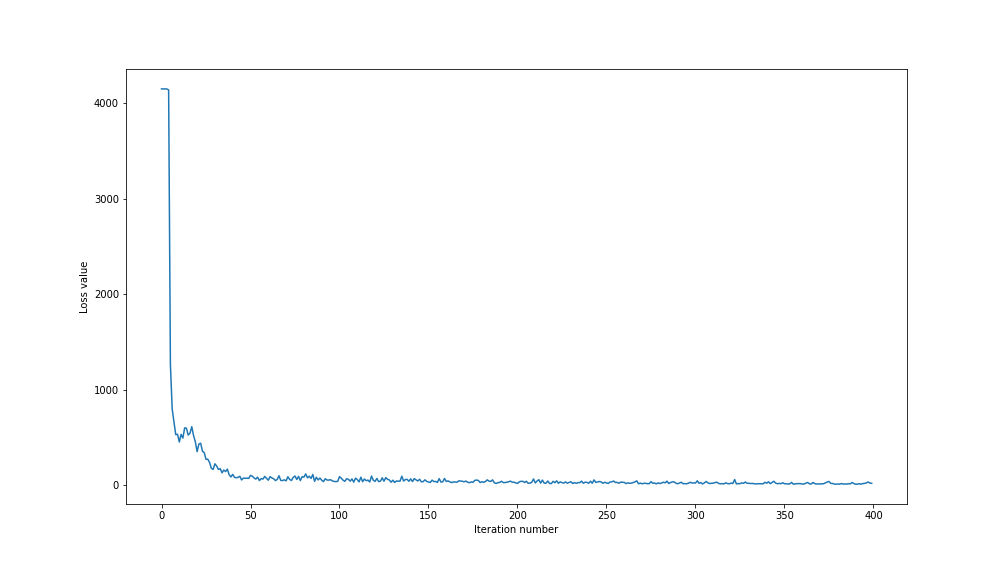
\includegraphics[width=10.1cm]{Images/det_train_loss.png}
        \caption{SGDを用いた$\det$の学習結果}
    \end{figure}
\end{Ex}
\section{Generative Adversarial Networks}
GAN$\cite{GAN}$は2014年にGoodfellowらによって提案された手法である. 
その後, WGAN, DCGANといった様々な亜種が登場し, 現在も様々な手法が提案されている.
冒頭でも述べたが, GANは警察と
泥棒の偽札造りに例えられる. $G$を泥棒, $D$を警察とした時, 以下の作業を繰り返すことで, 偽札の本物具合をあげていくといったものである.
\begin{enumerate}
    \item 泥棒$G$が偽札を作る.
    \item 警察$D$が偽札であると見破る.
    \item 泥棒$G$はなぜ,警察$D$に偽札であるとバレたのかを考え, より本物に近い偽札を作れるようになる.
\end{enumerate}
これらは以下のように$\min$-$\max$ゲームとして定式化される.
\subsection{GANの定式化}
この節では$D$は教師なしデータとする. また, データの確率分布を$\mathbb{P}_{data}$とする. 
\begin{Defi}[Generative Adversarial Networks]
    機械学習空間$\MLsp$を以下のように定義する$\cite{SNGAN}$. \\ 
    $\X\text{は}\RR^{d}\text{のコンパクト部分集合}$, $\Y = [0, 1]$, 
    \begin{align*}
        \Hil_{G} &= \{G:\mathcal{Z}\to\X~\mid G\text{はニューラルネット}\},\\
        \Hil_{D} &= \{D:\X\to\Y~\mid D\text{はニューラルネット}\},\\
        \Loss(G, D) &= \mathbb{E}_{x\sim \mathbb{P}_{data}}[\log D(x)] + \mathbb{E}_{x^{\prime}\sim \mathbb{P}_{G}}[\log(1 - D(x^{\prime}))],
    \end{align*}
    ここで, $\mathcal{Z}$は潜在空間と呼ばれる$\RR^d$の部分空間である. 
    また, $G\in\Hil_{1}$と確率分布$\mathbb{P}_{Z}$(一様分布や正規分布)に従う確率変数$Z:\Omega\to\mathcal{Z}$に対し, $G(Z)$が従う確率分布を$\mathbb{P}_{G}$とする. $G\in\Hil_{G}$を
    Generatorと呼び, $D\in\Hil_{D}$をDiscriminatorと呼ぶ.
    $\Hil = \Hil_{G}\times\Hil_{D}$とした時, 機械学習空間$\MLsp$を敵対的生成ネットワークという. 
\end{Defi}
GANの目的は, $\mathbb{P}_{G}$を$\mathbb{P}_{data}$に近づけることである. そのために, 以下のmin-maxゲームを解くことを考える. 
\begin{align*}
    \argmin_{G\in\Hil_{G}}\argmax_{D\in\Hil_{D}}\Loss(G, D).
\end{align*}
\begin{Rem}[GeneratorとDiscriminatorの役割について]
    Generator $G\in\Hil_{G}$の役割は, $z\in\mathcal{Z}$からデータとよく似た偽物$G(z)\in\X$を
    作成することである. 一方, Discriminator $D\in\Hil_{D}$の役割は, $x\in\X$が本物のデータなのかGeneratorが
    作った偽物であるのかを判断することである. そのために, $X\sim\mathbb{P}_{\X}$が本物である確率を学習する.
\end{Rem}
\begin{Defi}[最適Discriminator]
    $\MLsp$をGANとし, $G\in\Hil_{G}$とする. $D_{G}^{*}\in\Hil_{D}$が
    \begin{align*}
        \forall D\in\Hil_{D}, \Loss(D_{G}^{*}, G) \geq \Loss(D, G)
    \end{align*}
    を満たす時, $G$に関しての最適Discriminatorであるという.
\end{Defi}
\begin{Prop}[$\cite{GAN}$]\label{ODis}
    $\MLsp$をGANとし, $G\in\Hil_{G}$とする. この時, 最適Discriminatorは以下で与えられる.
    \begin{align*}
        D_{G}^{*}(x) = \frac{p_{data}(x)}{p_{data}(x) + p_{G}(x)},
    \end{align*}
    ここで, $p_{data}$は$\mathbb{P}_{data}$の確率密度関数であり, $p_{G}$は$\mathbb{P}_{G}$の確率密度関数である.
\begin{proof}
    期待値の計算から
    \begin{align*}
        \Loss(G, D) &= \int_{\X}p_{data}(x)\log(D(x))dx + \int_{\X}p_{G}(x)\log(1 - D(x))dx\\
                    &= \int_{\X}p_{data}(x)\log(D(x)) + p_{G}(x)\log(1 - D(x))dx
    \end{align*}
    を得る. ここで, 関数$F(a, b)(y) = a\log(y) + b\log(1 - y)$について, 
    \begin{align*}
        \argmax_{(a, b)\in\RR^{2}- \{(0, 0)\}}F(a, b)= \frac{a}{a + b}
    \end{align*}
    であることを用いれば主張が従う.
\end{proof}
\end{Prop}
この命題$\Ref{ODis}$より$\Hil_{G}$上の関数$C:\Hil_{G}\to\RR$が
\begin{align*}
    C(G) = \mathbb{E}_{x\sim\mathbb{P}_{data}}\left[ \log\frac{p_{data}(x)}{p_{data}(x) + p_{G}(x)} \right] + \mathbb{E}_{x^{\prime}\sim\mathbb{P}_{G}}\left[ \log\frac{p_{G}(x^{\prime})}{p_{data}(x^{\prime}) + p_{G}(x^{\prime})} \right]
\end{align*}
で定まる. 関数$C$を仮想訓練基準(virtual training criterion)と呼ぶ. 
\begin{Thm}[GANの最小性$\cite{GAN}$]
    $\MLsp$をGAN, $C$を仮想訓練基準とする. $C$が最小値$-\log4$を取るための必要十分条件は
    $\mathbb{P}_{data} = \mathbb{P}_{G}$となることである.
    \begin{proof}
        $\mathbb{P}_{data} = \mathbb{P}_{G}$とする. この時, 
        \begin{align*}
            C(G) &= \mathbb{E}_{x\sim\mathbb{P}_{data}}\left[ \log\frac{p_{data}(x)}{p_{data}(x) + p_{G}(x)} \right] + \mathbb{E}_{x^{\prime}\sim\mathbb{P}_{G}}\left[ \log\frac{p_{G}(x^{\prime})}{p_{data}(x^{\prime}) + p_{G}(x^{\prime})} \right]\\
                 &= \mathbb{E}_{x\sim\mathbb{P}_{data}}\left[ \log\frac{1}{2} \right] + \mathbb{E}_{x^{\prime}\sim\mathbb{P}_{G}}\left[ \log\frac{1}{2} \right]\\
                 &= -\log2 -\log2 = -\log4
        \end{align*}
        であるから, $C$は常に最小値$-\log4$をとる. 逆に$C$の最小値が$-\log4$であるとする. JSDをJensen-Shannon Divergenceとし, $C$を変形すると
        \begin{align*}
            C(G) = -\log4 + JSD\left(\mathbb{P}_{data}\|\mathbb{P}_{G}\right)
        \end{align*}
        となる. ここで$JSD\left(\mathbb{P}_{data}\|\mathbb{P}_{G}\right) = 0$と$\mathbb{P}_{data}=\mathbb{P}_{G}$は
        同値だから$\mathbb{P}_{data}=\mathbb{P}_{G}$である. 
    \end{proof}
\end{Thm}
これらからわかる通り, GANとはデータの確率密度関数をニューラルネットを用いて近似する機構である. 
\subsection{Instability of training GAN}
前節ではGANの定式化及び, いくつかの命題を証明した. ここではGANの学習の不安定性についてのべる. 詳しくは$\cite{PGAN}$を参照してほしい.
\begin{Thm}[The Perfect Discriminator Theorem]
    $\MLsp$をGANとし, $p_{data}$を$\mathbb{P}_{data}$の確率密度関数, $p_{G}$は$\mathbb{P}_{G}$の確率密度関数とする. この時, 
    \begin{align*}
        \exists M, P\subset\X:\text{compact s.t. }M\cap P = \emptyset, \text{supp}(p_{data})\subset M\text{ かつ }\text{supp}(p_{G})\subset P
    \end{align*}
    が成立するならば, 以下の性質を満たすsmoothな最適Discriminator $D_{G}^{*}$が存在する. 
    \begin{enumerate}
        \item $\mathbb{P}_{data}(D = 1) = 1\text{ かつ }\mathbb{P}_{G}(D = 0) = 1$
        \item $\forall x\in M\cup P, \nabla_{x}D_{G}^{*}(x) = 0$.
    \end{enumerate}
    \begin{proof}
        $P\cap M = \emptyset$だから, $\delta = d(P, M)$とすれば$\delta > 0$である. 
        ここで, 
        \begin{align*}
            \hat{M} &= \{x\in\X\mid d(x, M) \leq\delta/3\},\\
            \hat{P} &= \{x\in\X\mid d(x, P)\leq\delta/3\}
        \end{align*}
        と定義する. $M$, $P$がコンパクトであることと, $\delta$の定義より$\hat{M}$, $\hat{P}$は
        共にコンパクトであり, $\hat{M}\cap\hat{P}=\emptyset$である. したがって, Urysohn's smooth lemmaより
        \begin{align*}
            \exists D_{G}^{*}\in\Hil_{D}:\text{smooth s.t. } D_{G}^{*}|_{\hat{M}} = 1\text{ かつ }D_{G}^{*}|_{\hat{P}} = 0
        \end{align*}
        が成立する. 任意の$x\in\text{supp}(p_{data})$に対して, $D_{G}^{*}(x) = 1$だから, $\log D_{G}^{*}(x) = 0$である. 
        また, 任意の$x\in\text{supp}(p_{G})$に対して, $D_{G}^{*}(x) = 0$だから, $\log (1 - D_{G}^{*}(x)) = 0$である. これより
        $D_{G}^{*}$が最適Discriminatorであること, 及び1.が従う. また$D_{G}^{*}$は$M\cup P$上で定値写像だから2.が成立する. 
    \end{proof}
\end{Thm}
\begin{Defi}[Discriminatorノルム]
    $\MLsp$をGANとする. $D\in\Hil_{D}\subset C^{1}(\X)$に対して, 
    \begin{align*}
        \|D\| = \sup_{x\in\X}|D(x)| + \|\nabla_{x}D(x)\|_{2}
    \end{align*}
    とする. この時, $\|\cdot\|$の$\Hil_{D}$に制限したノルム$\|\cdot\|_{\Hil_{D}}$をDiscriminatorノルムという.
\end{Defi}
\begin{Thm}[Vanishing gradient on the Generator]
    $\MLsp$をGANとする. $G_{\theta}\in\Hil_{G}$とし, $p_{data}$を$\mathbb{P}_{data}$の確率密度関数, $p_{G}$は$\mathbb{P}_{G}$の確率密度関数とする. この時, 
    \begin{align*}
        \exists M, P\subset\X:\text{compact s.t. }M\cap P = \emptyset, \text{supp}(p_{data})\subset M\text{ かつ }\text{supp}(p_{G})\subset P
    \end{align*}
    が成立し, 
    \begin{align*}
        \exists M\in\RR^{+}\text{ s.t. }\forall \mathbb{E}_{z\sim\mathbb{P}_{Z}}[\|J_{\theta}G_{\theta}(z)\|_{2}^{2}] \leq M^{2}
    \end{align*}
    が成立するとする. この時, 任意の$\delta\in\RR^{+}-\{1\}$について, 
    \begin{align*}
        \forall D\in\Hil_{D}, \|D_{G} - D_{G}^{*}\|_{\Hil_{D}} <\delta \Longrightarrow\|\nabla_{\theta}\mathbb{E}_{z\sim\mathbb{P}_{Z}}[\log(1 - D(G_{\theta}(z)))]\|_{2} < M\frac{\delta}{1 - \delta}
    \end{align*}
    が成立する.
    \begin{proof}
        $\|\cdot\|^{2}$が凸であることと, Jensenの不等式より
        \begin{align*}
            \|\nabla_{\theta}\mathbb{E}_{z\sim\mathbb{P}_{Z}}[\log(1 - D(G_{\theta}(z)))]\|_{2}^{2} &\leq\mathbb{E}_{z\sim\mathbb{P}_{Z}}\left[ \frac{\|\nabla_{\theta}D(G_{\theta}(z))\|_{2}^{2}}{|1 - D(G_{\theta}(z))|^{2}} \right]\\
                                                                                                    &\leq\mathbb{E}_{z\sim\mathbb{P}_{Z}}\left[ \frac{\|\nabla_{x}D(G_{\theta}(z))\|_{2}^{2}\|J_{\theta}G_{\theta}(z)\|_{2}^{2}}{|1 - D(G_{\theta}(z))|^{2}} \right]\\
                                                                                                    &\leq\mathbb{E}_{z\sim\mathbb{P}_{Z}}\left[ \frac{(\|\nabla_{x}D^{*}(G_{\theta}(z))\|_{2} + \delta)^{2}\|J_{\theta}G_{\theta}(z)\|_{2}^{2}}{(|1 - D^{*}(G_{\theta}(z))| - \delta)^{2}} \right]\\
                                                                                                    &\leq\mathbb{E}_{z\sim\mathbb{P}_{Z}}\left[ \frac{\delta^{2}\|J_{\theta}G_{\theta}(z)\|_{2}^{2}}{(1 - \delta)^{2}} \right]\\
                                                                                                    &\leq M^{2}\frac{\delta^{2}}{(1 - \delta)^{2}}
        \end{align*}
        となる. 両辺の平方をとれば題意が従う. 
    \end{proof}
\end{Thm}
\begin{Cor}
    $\MLsp$をGANとする. $G_{\theta}\in\Hil_{G}$とし, $p_{data}$を$\mathbb{P}_{data}$の確率密度関数, $p_{G}$は$\mathbb{P}_{G}$の確率密度関数とする. 先の定義の仮定条件の元で, 
    \begin{align*}
        \lim_{\|D - D^{*}\|_{\Hil_{D}}\to0}\nabla_{\theta}\mathbb{E}_{z\sim\mathbb{P}_{Z}}[\log(1 - D(G_{\theta}(z)))] = 0
    \end{align*}
    が成立する. 
\end{Cor}
これらの定理・系からDiscriminatorが最適解に近づけば近づくほど, Generatorの勾配が0に近づき学習が安定しないことがわかる.
\subsection{Stabilization of training GAN}
GANの学習を安定化させるために, Gradient Penalty\cite{WGAN}やSpectral Normalization\cite{SNGAN}などの手法が提案されている. 
今回は, パラメータ行列の特異値を利用するSpectral Normalizationを紹介する. $\MLsp$をGANとする. 
$f$を$D$から最終層の活性化関数$\mathcal{A}$を省いたものとする(すなわち$D = \mathcal{A}\circ f$.)
\begin{Prop}[\cite{SNGAN}]
    $f$の各層の活性化関数のLipschitzノルムが1であるとする. この時, 
    \begin{align*}
        \|f\|_{Lip} \leq \prod_{k = 1}^{K + 1}\|W_{k}\|_{op} 
    \end{align*}
    が成立する. ここで$g_{k} = \eta(W_{k}x + b_{k})$とした時, 
    $f(x) = W_{K + 1}^{\top}g_{K}\circ\cdots\circ g_{1}(x) + b$
    とする. ここで, $\|f\|_{Lip}$はLipschitzノルム, $\|\cdot\|_{op}$で行列の作用素ノルムを表す. 
    \begin{proof}
        Lipschitzノルムの性質と$\|g_{k}\|_{Lip} = \|W_{k}\|_{op}$より,
        \begin{align*}
            \|f\|_{Lip} &\leq \displaystyle \prod_{k = 1}^{K} \|g_{k}\|_{Lip}\\
                        & \leq \displaystyle \prod_{k = 1}^{K} \|\eta_{k}\|_{Lip}\|W_{k}\|_{op}\\
                        & = \displaystyle \prod_{k = 1}^{K} \|W_{k}\|_{op}.
        \end{align*}
    \end{proof}
\end{Prop}
したがって, 各層のパラメータ$W_{K}$の各成分を$\|W_{k}\|_{op}$で割れば, $\|f\|_{Lip}\leq 1$とすることができる.
この手法を, Spectral Normalization と呼ぶ. 
\begin{Defi}[SNGAN\cite{SNGAN}]
    $\MLsp$をGANのML空間とする. この時, Spectral Normalizationを用いて
    \begin{align*}
        \argmin_{G\in\Hil_{G}}\argmax_{D\in\Hil_{D}, \|f\|_{Lip}\leq 1}\Loss(G, D).
    \end{align*}
    を解く問題をSNGANという. ここで, $f$は$D$から最終層の活性化関数$\mathcal{A}$を
    省いたものである(すなわち$D = \mathcal{A}\circ f$.)
\end{Defi}
\subsection{GANの応用}
最後に言葉のみではあるがGANの応用であるCycle-GAN\cite{CGAN}やGameGAN\cite{GGAN}について紹介する. 
Cycle-GANは2つのGANを用意することにより, 画像の変換をすることができるモデルである. 例えば, 
夏の画像を冬の画像に変えたりすることができる. GameGANはゲーム環境のようにリアルで複雑な環境の生成を目指したGANであり,  
論文中ではPac-Manの生成に成功している, 
\section{Conclusion}
今回は, 近年の深層学習の大きな結果である敵対的生成ネットワークについて
のべた. しかしながら, 本稿は2017年までの理論解析部分しか追えておらず, 
2020, 2021年の話題についておまり触れられなかったことが心残りである. しかし, 
この記事を書くにあたり, もう一度文献を読み直し, 機械学習への理解を深めることができた
ことはとてもよかった. \\
\indent 最後にはなるが, 学部4年間の間で支えていただいた, 友人, 先生方の皆様にはこの場で感謝を申し上げる. 
引き続き大学院でも頑張っていきたい. 
\begin{thebibliography}{20}
    \bibitem{MLR} darden. 多クラス分類ロジスティック回帰. \\
    http://darden.hatenablog.com/entry/2018/01/25/222201. Pythonと機械学習, 2018
    \bibitem{Adam} Diederik P. Kingma and Jimmy Ba. Adam: A Method for Stochastic Optimization. 
    International Conference on Learning Representations, 2015.
    \bibitem{UAT} G. Cybenko. Approximation by Superpositions of a Sigmoidal Function. Mathmatics of control, signal and systems. vol. 2, no. 4, 1989
    \bibitem{GAN} Ian J. Goodfellow, Jean Pouget-Abadie, Mehdi Mirza, Bing Xu, David Warde-Farley, Sherjil Ozair, Aaron Courville and Yoshua Bengio. 
    Generative adversarial nets. In Advances in Neural Information Processing Systems, 2014.
    \bibitem{CGAN} Jun-Yan Zhu, Taesung Park, Phillip Isola and Alexei A. Efros. Unpaired Image-to-Image Translation using Cycle-Consistent Adversarial Networks.
                    International Conference on Computer Vision. 2017.
    \bibitem{PGAN}Martin Arjovsky and Leon Bottou. Towards Principled Methods for Training Generative Adversarial Networks.
    International Conference on Learning Representations, 2017.
    \bibitem{WGAN} Martin Arjovsky, Soumith Chintala and Leon Bottou. Wasserstein GAN.
    International Conference on Learning Representations, 2017.
    \bibitem{SNGAN}Takeru Miyato, Toshiki Kataoka, Masanori Koyama and Yuichi Yoshida. Spectral Normalization for Generative Adversarial Networks. 
    International Conference on Learning Representations, 2018.
    \bibitem{DUAT} mochimochidog. ニューラルネットワークの普遍性定理. \\
    https://qiita.com/mochimochidog/items/ca04bf3df7071041561a. Qiita, 2020.
    \bibitem{} Preferred Networks. ディープラーニング入門 Chainer チュートリアル.\\
    https://tutorials.chainer.org/ja/index.html, 2019.
    \bibitem{GGAN} Seung Wook Kim, Yuhao Zhou, Jonah Philion, Antonio Torralba and Sanja Fidler.
    Learning to Simulate Dynamic Environments With GameGAN.  Conference on Computer Vision and Pattern Recognition. 2020.
\end{thebibliography}


\end{document}

